\documentclass{tufte-handout}

\usepackage[french]{babel}
\usepackage[utf8]{inputenc}
\usepackage[T1]{fontenc}
\usepackage{amsmath, amsthm, amsfonts}
\usepackage{siunitx}
\usepackage{tikz}
\usepackage{hyperref}
%\usepackage[backend=biber, autocite=footnote]{biblatex}
\usepackage{xcolor}
\usepackage{caption}
\usepackage{booktabs}
\usepackage{mathtools}

\tikzset{>=latex}
\usetikzlibrary{calc,decorations.pathreplacing}
\sisetup{locale=FR, per-mode=symbol}

\newcommand{\abs}[1]{\left| #1 \right|}
%\renewcommand{\vec}[1]{\ensuremath{\overrightarrow{\boldsymbol{\mathrm{ #1 }}}}}
\newcommand{\rhat}{\vec{\hat{r}}}
\newcommand{\xhat}{\vec{i}}
\newcommand{\yhat}{\vec{j}}
\newcommand{\zhat}{\vec{k}}
\newcommand{\real}{\mathbb{R}}
\newcommand{\der}[2]{\frac{\mathrm{d}#1}{\mathrm{d}#2}}
\newcommand{\pder}[2]{\frac{\partial #1}{\partial #2}}
\newcommand{\dif}{\mathrm{d}}
\newcommand{\ddif}{\,\mathrm{d}}
\newcommand{\grad}{\vec{\nabla}}
\newcommand{\exemple}[1]{\begin{fullwidth}#1\end{fullwidth}}
\newcommand{\norm}[1]{\lVert #1 \rVert}
\newcommand{\vu}{\vec{u}}
\newcommand{\vv}{\vec{v}}
\newcommand{\vr}{\vec{r}}
\newcommand{\va}{\vec{a}}
\newcommand{\vF}{\vec{F}}
\newcommand{\vecxyz}[3]{#1 \xhat + #2 \yhat + #3 \zhat}
\newcommand{\vecxy}[2]{#1 \xhat + #2 \yhat}

\theoremstyle{definition}
\newtheorem*{defn}{Definition}



\title{Exercices sur le MRUA}
\date{}

\begin{document}

\maketitle
\vspace{0.5cm}

\section{Exercice I -- Freinage en voiture}

Un conducteur dans sa voiture voit un piéton à \SI{30}{\meter} devant lui.  À
ce moment, il décide d'appliquer les freins pour tenter d'éviter de frapper le
piéton.  À partir du moment où il appuie sur la pédale de frein, on suppose que
son accélération a un module constant.  Il parvient à arrêter sa voiture juste
avant d'atteindre le piéton.

\begin{marginfigure}
  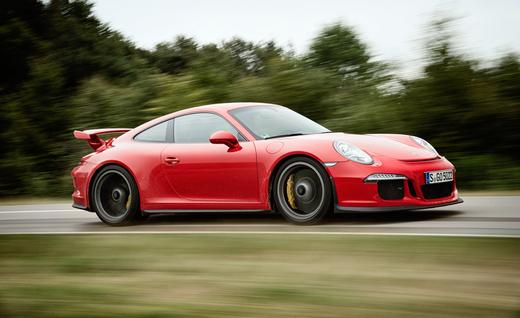
\includegraphics[scale=0.3]{2014porsche911gt3.jpg}
  \caption{Une Porsche 911 GT3 2014 peut freiner avec une accélération de
    module \SI{11.9}{\meter\per\second\squared}.}
  \label{fig:porsche}
\end{marginfigure}

En général, entre le moment où un conducteur décide de freiner et le moment où
il commence à appuyer sur la pédale de frein, il s'écoule \SI{1.3}{\second}.
On suppose que notre conducteur est un pilote professionnel et que son temps de
réaction est plutôt \SI{1}{s}.

\begin{marginfigure}
  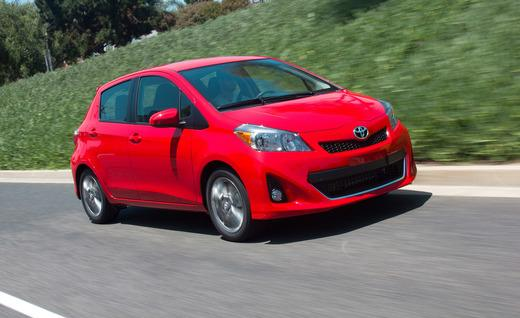
\includegraphics[scale=0.3]{2012toyota_yaris.jpg}
  \caption{Une Toyota Yaris 2012 peut freiner avec une accélération de
    module \SI{9.29}{\meter\per\second\squared}.  Les modèles plus lourds,
    comme la Prius V 2013 n'atteignent que des accélérations de module
    \SI{8.41}{\meter\per\second\squared}.}
  \label{fig:porsche}
\end{marginfigure}

La majorité des voitures ont un module d'accélération maximal lors
d'un freinage situé entre \SI{7.5}{\meter\per\second\squared} et
\SI{9.8}{\meter\per\second\squared}.  On suppose que notre conducteur possède
une excellente voiture sport munie de pneus neufs et d'excellente qualité.
Grâce à cela, il peut freiner avec une accélération de module
\SI{11.9}{\meter\per\second\squared}.

\begin{enumerate}[a]
  \item Déterminer la vitesse à laquelle la voiture se déplaçait
    lorsque le conducteur a aperçu le piéton.
  \item Sur une chaussée mouillée, le module maximal de l'accélération est
    réduit de \SI{35}{\percent}.  Si la voiture se déplaçait à la vitesse
    calculée en (a), à quelle vitesse aurait-elle percuté le piéton sur une
    chaussée mouillée?
  \item Supposons à nouveau que la chaussée est sèche.  Si le conducteur allait
    \SI{5}{\kilo\meter\per\hour} plus vite que la vitesse calculée en (a), à
    quelle vitesse aurait-il percuté le piéton?
\end{enumerate}

\marginnote{Les données sur les accélérations et les images proviennent du site
  \url{http://www.caranddriver.com/list-reviews-instrumented-tests/}. Le site
  contient une description détaillée du protocole expérimental utilisé pour
  faire les mesures de freinage.

  Le temps de réaction pour le freinage provient du dépliant \emph{Sur la
  route, prenez le temps de ralentir} publié par la SAAQ et disponible à
  l'adresse
  \url{http://www.saaq.gouv.qc.ca/publications/prevention/route_ralentir.pdf}.

  L'impact d'une chaussée mouillé a été déterminé à partir des données fournies
  par la police fédérale australienne
  \url{http://www.police.act.gov.au/roads-and-traffic/speeding/stopping-distances-explained.aspx}.
}

\subsection{Solution}

\begin{enumerate}[a]
  \begin{marginfigure}
    \begin{tikzpicture}[scale=1]
      \draw[->] (0, 0) -- (6, 0) node[below] {$x$};
      \draw (0.3, 0) -- (0.3, -0.1) node[below] {$x_0 = 0$};
      \draw (2.2, 0) -- (2.2, -0.1) node[below] {$x_1$};
      \draw (5, 0) -- (5, -0.1) node[below] {$x_2$};
      \draw (5, 1) circle (0.1);
      \draw (5, 0.9) -- (5, 0.4) -- (4.8, 0.2)
            (5, 0.4) -- (5.2, 0.2)
            (5, 0.7) -- (4.8, 0.9)
            (5, 0.7) -- (5.2, 0.9);
    \draw (0.6, 0.25) circle (0.1);
    \draw (0, 0.25) circle (0.1);
    \draw[fill=white] (-0.2, 0.3) -- (0.8, 0.3) -- (0.75, 0.4) -- (0.4, 0.5) -- (0, 0.5) -- cycle;
    \draw[->, very thick] (0.9, 0.3) -- (1.5, 0.3) node[above] {$\vec{v}_0$};
    \draw [decorate,decoration={brace,amplitude=10pt,raise=4pt},yshift=0pt] (0.3, 1) -- (2.18, 1);
    \node at (1.2, 1.8) {MRU};
    \draw [decorate,decoration={brace,amplitude=10pt,raise=4pt},yshift=0pt] (2.22, 1) -- (5, 1);
    \node at (3.6, 1.8) {MRUA};
    \end{tikzpicture}
  \end{marginfigure}
  \item On décompose le temps d'arrêt en deux parties: le temps entre le moment
    où le conducteur voit le piéton ($t_0 = \SI{0}{\second}$) et celui où il
    appuie sur le frein ($t_1$), et le temps entre le moment où il appuie sur
    le frein et celui où la voiture arrête ($t_2$).  Entre $t_0$ et $t_1$, la
    voiture avance à vitesse constante et donc son mouvement est rectiligne
    uniforme.  Entre $t_1$ et $t_2$, le conducteur freine et la voiture est
    donc en mouvement rectiligne uniformément accéléré.

    Soit $x_0$, $x_1$ et $x_2$ les positions aux temps $t_0$, $t_1$ et $t_2$
    respectivement; soit $v_0$ le module de la vitesse initiale.  

    On cherche $v_{0}$.

    On connaît les quantités suivantes:
    \begin{enumerate}[i.]
      \item $v_{2x} = \SI{0}{\meter\per\second}$
      \item $x_0 = \SI{0}{\meter}$
      \item $x_2 = \SI{30}{\meter}$
      \item $t_0 = \SI{0}{\second}$
      \item $t_1 = \SI{1}{\second}$
    \end{enumerate}

    \begin{marginfigure}
    \begin{tikzpicture}[scale=1]
      \draw[->] (0, 0) -- (6, 0) node[below] {$t$};
      \draw[->] (0, 0) -- (0, 5) node[left] {$v_{x}$};
      \draw[thick] (0, 3) node[left] {$v_{0x}$} -- (2, 3) -- (5, 0);
      \draw[dashed] (2, 3) -- (2, 0) node[below] {$t_1$};
      \node[below] at (5, 0) {$t_2$};
    \end{tikzpicture}
    \end{marginfigure}

    La position finale de la voiture est la même que la position du piéton.
    Puisque la position initiale est \SI{0}{\meter}, le déplacement lors du MRU
    plus le déplacement lors du MRUA doit être égal à $x_2$:
    \[
      x_2 = \Delta x_\mathrm{MRU} + \Delta x_\mathrm{MRUA}
    \]
    Pour le MRU, l'intervalle de temps est entre $0$ et $t_1$ donc
    \begin{align*}
      \Delta x_\mathrm{MRU} = v_{0x} t_1
    \end{align*}
    Pour le MRUA, l'intervalle de temps est entre $t_1$ et $t_2$.
    \begin{align*}
      \Delta x_\mathrm{MRUA} = v_{0x} (t_2 - t_1) + \frac{1}{2} a_x (t_2 -
                               t_1)^2
    \end{align*}
    En combinant les deux on obtient
    \begin{align}
      x_2 &= v_{0x} t_1 + v_{0x} (t_2 - t_1) + \frac{1}{2} a_x (t_2 -
                               t_1)^2 \label{eqn:car1}
    \end{align}
    On a une équation avec deux inconnues $v_{0x}$ et $t_2$.  Il nous faut une
    autre équation pour résoudre le problème.  La seule information que nous
    n'avons toujours par utilisée est le fait que la vitesse finale est nulle.
    On sait que la deuxième partie du mouvement est un MRUA donc
    \begin{equation}
      v_{2x} = v_{0x} + a_x (t_2 - t_1)
      \label{eqn:car2}
    \end{equation}
    et cette expression se simplifie parce que $v_{2x} =
    \SI{0}{\meter\per\second}$:
    \begin{equation}
      \SI{0}{\meter\per\second} = v_{0x} + a_x (t_2 - t_1)
      \label{eqn:car3}
    \end{equation}
    On peut isoler $t_2 - t_1$ dans l'équation \ref{eqn:car3} et substituer dans
    l'équation \ref{eqn:car1}.
    \begin{align*}
      t_2 - t_1 &= \frac{- v_{0x}}{a_x} \\
      x_2 &= v_{0x} t_1 + v_{0x} \frac{- v_{0x}}{a_x} + \frac{1}{2} a_x
             \left(\frac{- v_{0x}}{a_x}\right)^2 \\
          &= v_{0x} t_1 - \frac{1}{2} \frac{v_{0x}^2}{a_x}
    \end{align*}
    Cette équation est quadratique en $v_{0x}$.  On peut donc la résoudre avec
    la formule quadratique.  Tout d'abord on la récrit dans la forme habituelle 
    \[
      \frac{1}{2a_x} v_{0x}^2 - t_1v_{0x} + x_2 = 0
    \]
    puis on applique la formule
    \begin{align*}
      v_{0x} &= \frac{t_1 \pm \sqrt{t_1^2 - 4x_2 / (2a_x)}}{1/a_x} \\
             &= a_x\left( t_1 \pm \sqrt{t_1^2 - 2x_2 / a_x} \right)
    \end{align*}
    On sait que la composante de la vitesse est positive alors que la
    composante de l'accélération est négative, par conséquent, seule la
    solution avec le ``$-$'' est physiquement possible.
    \begin{align*}
      v_{0x} &= a_x\left( t_1 - \sqrt{t_1^2 - 2x_2 / a_x} \right) \\
             &= \SI{17.3508}{\meter\per\second} \\
             &= \SI{62.4629}{\kilo\meter\per\hour}
    \end{align*}
    \[
      \boxed{v_{0x} = \SI{17.4}{\meter\per\second}}
    \]


  \item Si la chaussée est mouillée, le module de l'accélération diminue de
    \SI{35}{\percent}, donc
    \[
      a_{mx} = \num{0.65} a_x = -\SI{7.735}{\meter\per\second\squared}
    \]
    On connaît la vitesse initiale
    \[
      v_{0x} = \SI{17.3508}{\meter\per\second}
    \]
    et on cherche la vitesse finale, c'est-à-dire lorsque la voiture atteint le
    piéton.

    Pendant le MRU, la voiture fait un déplacement
    \begin{align*}
      \Delta x_\mathrm{MRU} = v_{0x} t_{1}.
    \end{align*}
    Lorsque le chauffeur commence à appuyer sur les freins, il est donc à la
    position $x_i = v_{0x} t_{1}$.

    Lors du MRUA, la vitesse en fonction du temps est donnée par
    \[
      v_x = v_{0x} + a_{mx} t'
    \]
    où $t'$ est le temps depuis le début du MRUA (donc $t' = t - t_1$).  Si on
    élève cette expression au carré, on obtient
    \begin{align*}
      v_x^2 &= \left( v_{0x} + a_{mx} t' \right)^2 \\
            &= v_{0x}^2 + 2v_{0x} a_{mx} t' + a_x^2 t'^2 \\
            &= v_{0x}^2 + 2a_{mx}\left(v_{0x} t' + \frac{1}{2} a_{mx} t'^2\right) \\
      v_x^2 &= v_{0x}^2 + 2a_{mx}\left( x - x_i \right) \\
    \end{align*}
    Si on applique cette relation à l'instant où la voiture frappe le piéton,
    $x = \SI{30}{\meter}$ et $v_{x}$ est la vitesse recherchée.
    \begin{align*}
      v_x &= \sqrt{v_{0x}^2 + 2a_{mx}\left( x - x_i \right)} \\
          &= \sqrt{v_{0x}^2 + 2a_{mx}\left( x - v_{0x}t_1 \right)} \\
          &= \SI{10.2648}{\meter\per\second} \\
          &= \SI{36.9534}{\kilo\meter\per\second}
    \end{align*}
    \[
      \boxed{v_x = \SI{10.3}{\meter\per\second}}
    \]


  \item Ici, la vitesse initiale est
    \begin{align*}
      v_{0x} &= \SI{62.4629}{\kilo\meter\per\hour} +
                \SI{5}{\kilo\meter\per\hour} \\
             &= \SI{18.7397}{\meter\per\second}
    \end{align*}
    On peut appliquer exactement la même formule qu'à la question précédente.
    \begin{align*}
      v_x &= \sqrt{v_{0x}^2 + 2a_{x}\left( x - v_{0x}t_1 \right)} \\
          &= \SI{9.12037}{\meter\per\second} \\
          &= \SI{32.8333}{\kilo\meter\per\second}
    \end{align*}
    \[
      \boxed{v_x = \SI{9.12}{\meter\per\second}}
    \]

\end{enumerate}

\newpage

\section{Exercice II -- Partie de football}

Un joueur de football des Alouettes court vers la zone de touche de l'équipe
adverse, les Stampeders, à une vitesse constante de \SI{10}{\meter\per\second}.
Lorsqu'il franchit la ligne de $40$ verges de son côté du terrain, un
coéquipier lui passe le ballon.  \SI{0.8}{\second} après que le joueur des
Alouettes ait reçu le ballon, un joueur des Stampeders situé en face, à la
ligne de $20$ verges du côté des Stampeders, se lance vers lui à partir du
repos.  On suppose que le joueur des Stampeders a une accélération constante.

\begin{marginfigure}
  \begin{tikzpicture}[scale=0.9]
    \fill[green!40] (-0.6, 0) rectangle (6.6, 3);
    \draw[opacity=0.8, fill=green!60!black] (0, 0) rectangle (6, 3);
    \draw[thick, green!20!white, dashed] (3, 0) -- node {$5\,0$} (3, 3);
    \foreach \i in {1, 2, ..., 4} {
      \draw[thick, green!20!white, dashed] (0.6*\i, 0) -- node {$\i\,0$} (0.6*\i, 3);
      \draw[thick, green!20!white, dashed] (6-0.6*\i, 0) -- node {$\i\,0$} (6-0.6*\i, 3);
    }
    \node[rotate=90, green!40!black] at (-0.3, 1.5) {ALOUETTES};
    \node[rotate=-90, green!40!black] at (6.3, 1.5) {STAMPEDERS};
    \node[circle, fill=blue!25, thick, draw=blue!50!white] (A) at (2.4, 0.8) {$A$};
    \node[circle, fill=red!25, thick, draw=red!50!white] at (4.8, 0.8) {$S$};
    \draw[very thick, ->] (A) -- ++(1, 0) node[below] {$\vec{v}_{A}$};
  \end{tikzpicture}
  \caption{Position des deux joueurs au moment où le joueur des Alouettes
    reçoit le ballon.  Le joueur des Alouettes est représenté par un $A$ et
    celui des Stampeders par un $S$.}
  \label{fig:football}
\end{marginfigure}

Si les deux joueurs entrent en collision \SI{2}{\second} après le départ du
joueur des Stampeders déterminer les quantités suivantes:

\begin{enumerate}
  \item l'accélération du joueur des Stampeders;
  \item la vitesse du joueur des Stampeders lors de la collision;
  \item la position des joueurs lors de la collision;
\end{enumerate}

\textit{Note: Une verge est égale à \SI{0.9144}{\meter}.}

\subsection{Solution}

Posons que le temps auquel le joueur $A$ reçoit le ballon est $t =
\SI{0}{\second}$.  Le joueur $A$ est toujours en mouvement rectiligne uniforme
alors que je joueur $S$ est au repos pendant \SI{0.8}{\second} puis il est en
mouvement rectiligne uniformément accéléré pour la suite.  On pose aussi que la
position initiale de $A$ est à $x = \SI{0}{\meter}$.

Soit $x_A$ la position de $A$. On sait que
\[
  x_A(t) = v_{Ax} t.
\]
Dans le cas de $S$, sa position ne commence à changer qu'à partir de $t =
\SI{0.8}{\second}$.  Sa position initiale est $x_{S0} = 40\, \mathrm{verges}$.
Une fois qu'il a commencé à courir, sa position est donnée par un MRUA, mais il
faut tenir compte du fait que le temps pendant lequel il a couru est en réalité
$t - \SI{0.8}{\second}$:
\[
  x_S(t) = x_{S0} + v_{S0} (t - \SI{0.8}{\second})
           + \frac{1}{2} a_x (t - \SI{0.8}{\second})^2
\]
Puisqu'il part du repos, sa vitesse initiale est nulle et donc
\[
  x_S(t) =  x_{S0} + \frac{1}{2} a_x (t - \SI{0.8}{\second})^2
\]

La collision a lieu lorsque la position des deux joueurs est la même, i.e.:
\begin{align*}
  x_A &= x_S \\
  v_{Ax} t_\mathrm{collision} &= x_{S0} + \frac{1}{2} a_x (t_\mathrm{collision} - \SI{0.8}{\second})^2
\end{align*}
et on sait que la collision a lieu à $t_\mathrm{collision} = \SI{2.8}{s}$.
L'équation précédente ne contient qu'une seule inconnue, soit l'accélération.
Un peu d'algèbre donne
\[
  a_x = \frac{2\left(v_{Ax} t_\mathrm{collision} - x_{S0}\right)}
             {(t_\mathrm{collision} - \SI{0.8}{\second})^2}
\]
\[
  \boxed{a_x = \SI{-4.29}{\meter\per\second\squared}}
\]

Une fois qu'on connaît l'accélération, il est facile de déterminer la vitesse
du joueur des Stampeders:
\begin{align*}
  v_{Sfx} = a_x (t_\mathrm{collision} - \SI{0.8}{\second})
\end{align*}
\[
  \boxed{v_{Sfx} = \SI{-8.58}{\meter\per\second}}
\]

On peut calculer la position de la collision simplement à partir de la vitesse
du joueur $A$ et du temps avant que la collision ne se produise.
\begin{align*}
  x_\mathrm{collision} &= v_{Ax} t_\mathrm{collision}
\end{align*}
\[
  \boxed{x_\mathrm{collision} = \SI{28.0}{\meter} = \num{30.6}\,\mathrm{verges}}
\]
Autrement dit, le joueur des Alouettes aura tout juste le temps de franchir la
ligne de \num{30} verges du côté des Stampeders avant d'être plaqué.

\end{document}
